\documentclass[ignorenonframetext,]{beamer}
\setbeamertemplate{caption}[numbered]
\setbeamertemplate{caption label separator}{: }
\setbeamercolor{caption name}{fg=normal text.fg}
\beamertemplatenavigationsymbolsempty
\usepackage{lmodern}
\usepackage{amssymb,amsmath}
\usepackage{ifxetex,ifluatex}
\usepackage{fixltx2e} % provides \textsubscript
\ifnum 0\ifxetex 1\fi\ifluatex 1\fi=0 % if pdftex
\usepackage[T1]{fontenc}
\usepackage[utf8]{inputenc}
\else % if luatex or xelatex
\ifxetex
\usepackage{mathspec}
\else
\usepackage{fontspec}
\fi
\defaultfontfeatures{Ligatures=TeX,Scale=MatchLowercase}
\fi
\usetheme{Madrid}
\usecolortheme{udesc}
% use upquote if available, for straight quotes in verbatim environments
\IfFileExists{upquote.sty}{\usepackage{upquote}}{}
% use microtype if available
\IfFileExists{microtype.sty}{%
\usepackage{microtype}
\UseMicrotypeSet[protrusion]{basicmath} % disable protrusion for tt fonts
}{}
\newif\ifbibliography
\usepackage{color}
\usepackage{fancyvrb}
\newcommand{\VerbBar}{|}
\newcommand{\VERB}{\Verb[commandchars=\\\{\}]}
\DefineVerbatimEnvironment{Highlighting}{Verbatim}{commandchars=\\\{\}}
% Add ',fontsize=\small' for more characters per line
\usepackage{framed}
\definecolor{shadecolor}{RGB}{248,248,248}
\newenvironment{Shaded}{\begin{snugshade}}{\end{snugshade}}
\newcommand{\KeywordTok}[1]{\textcolor[rgb]{0.13,0.29,0.53}{\textbf{{#1}}}}
\newcommand{\DataTypeTok}[1]{\textcolor[rgb]{0.13,0.29,0.53}{{#1}}}
\newcommand{\DecValTok}[1]{\textcolor[rgb]{0.00,0.00,0.81}{{#1}}}
\newcommand{\BaseNTok}[1]{\textcolor[rgb]{0.00,0.00,0.81}{{#1}}}
\newcommand{\FloatTok}[1]{\textcolor[rgb]{0.00,0.00,0.81}{{#1}}}
\newcommand{\ConstantTok}[1]{\textcolor[rgb]{0.00,0.00,0.00}{{#1}}}
\newcommand{\CharTok}[1]{\textcolor[rgb]{0.31,0.60,0.02}{{#1}}}
\newcommand{\SpecialCharTok}[1]{\textcolor[rgb]{0.00,0.00,0.00}{{#1}}}
\newcommand{\StringTok}[1]{\textcolor[rgb]{0.31,0.60,0.02}{{#1}}}
\newcommand{\VerbatimStringTok}[1]{\textcolor[rgb]{0.31,0.60,0.02}{{#1}}}
\newcommand{\SpecialStringTok}[1]{\textcolor[rgb]{0.31,0.60,0.02}{{#1}}}
\newcommand{\ImportTok}[1]{{#1}}
\newcommand{\CommentTok}[1]{\textcolor[rgb]{0.56,0.35,0.01}{\textit{{#1}}}}
\newcommand{\DocumentationTok}[1]{\textcolor[rgb]{0.56,0.35,0.01}{\textbf{\textit{{#1}}}}}
\newcommand{\AnnotationTok}[1]{\textcolor[rgb]{0.56,0.35,0.01}{\textbf{\textit{{#1}}}}}
\newcommand{\CommentVarTok}[1]{\textcolor[rgb]{0.56,0.35,0.01}{\textbf{\textit{{#1}}}}}
\newcommand{\OtherTok}[1]{\textcolor[rgb]{0.56,0.35,0.01}{{#1}}}
\newcommand{\FunctionTok}[1]{\textcolor[rgb]{0.00,0.00,0.00}{{#1}}}
\newcommand{\VariableTok}[1]{\textcolor[rgb]{0.00,0.00,0.00}{{#1}}}
\newcommand{\ControlFlowTok}[1]{\textcolor[rgb]{0.13,0.29,0.53}{\textbf{{#1}}}}
\newcommand{\OperatorTok}[1]{\textcolor[rgb]{0.81,0.36,0.00}{\textbf{{#1}}}}
\newcommand{\BuiltInTok}[1]{{#1}}
\newcommand{\ExtensionTok}[1]{{#1}}
\newcommand{\PreprocessorTok}[1]{\textcolor[rgb]{0.56,0.35,0.01}{\textit{{#1}}}}
\newcommand{\AttributeTok}[1]{\textcolor[rgb]{0.77,0.63,0.00}{{#1}}}
\newcommand{\RegionMarkerTok}[1]{{#1}}
\newcommand{\InformationTok}[1]{\textcolor[rgb]{0.56,0.35,0.01}{\textbf{\textit{{#1}}}}}
\newcommand{\WarningTok}[1]{\textcolor[rgb]{0.56,0.35,0.01}{\textbf{\textit{{#1}}}}}
\newcommand{\AlertTok}[1]{\textcolor[rgb]{0.94,0.16,0.16}{{#1}}}
\newcommand{\ErrorTok}[1]{\textcolor[rgb]{0.64,0.00,0.00}{\textbf{{#1}}}}
\newcommand{\NormalTok}[1]{{#1}}
\usepackage{graphicx,grffile}
\makeatletter
\def\maxwidth{\ifdim\Gin@nat@width>\linewidth\linewidth\else\Gin@nat@width\fi}
\def\maxheight{\ifdim\Gin@nat@height>\textheight0.8\textheight\else\Gin@nat@height\fi}
\makeatother
% Scale images if necessary, so that they will not overflow the page
% margins by default, and it is still possible to overwrite the defaults
% using explicit options in \includegraphics[width, height, ...]{}
\setkeys{Gin}{width=\maxwidth,height=\maxheight,keepaspectratio}

% Prevent slide breaks in the middle of a paragraph:
\widowpenalties 1 10000
\raggedbottom

\AtBeginPart{
\let\insertpartnumber\relax
\let\partname\relax
\frame{\partpage}
}
\AtBeginSection{
\ifbibliography
\else
\let\insertsectionnumber\relax
\let\sectionname\relax
\frame{\sectionpage}
\fi
}
\AtBeginSubsection{
\let\insertsubsectionnumber\relax
\let\subsectionname\relax
\frame{\subsectionpage}
}

\setlength{\parindent}{0pt}
\setlength{\parskip}{6pt plus 2pt minus 1pt}
\setlength{\emergencystretch}{3em}  % prevent overfull lines
\providecommand{\tightlist}{%
\setlength{\itemsep}{0pt}\setlength{\parskip}{0pt}}
\setcounter{secnumdepth}{0}
%%%%%%%%%%%%%%%%%%%%%%%%%%%%%%%%%%%%%%%%%%%%%%%%%%%%%%%%%%%%%%%%%%%%%%%%%%%%%%%%%%%%%%%%%%%%%%
% Template Beamer 
% Based on MIT Beamer Template e Senac
% Cores verde e vermelho tentam seguir o padrão visual da Udesc
%%%%%%%%%%%%%%%%%%%%%%%%%%%%%%%%%%%%%%%%%%%%%%%%%%%%%%%%%%%%%%%%%%%%%%%%%%%%%%%%%%%%%%%%%%%%%% 

\usepackage{graphicx,url}
\usepackage[brazil]{babel}   
\usepackage{textpos}

\batchmode
% \usepackage{pgfpages}
% \pgfpagesuselayout{4 on 1}[letterpaper,landscape,border shrink=5mm]
\usepackage{amsmath,amssymb,enumerate,epsfig,bbm,calc,color,ifthen,capt-of}

%-------------------------Declara figura do Logo-----------------------------------------------------
\pgfdeclareimage[height=0.8cm]{Marca_Udesc}{Marca_Udesc.pdf}
%\logo{\pgfuseimage{Marca_Udesc}\vspace*{7.0cm}}

%-------------------------Este código faz o menuzinho bacana na parte superior do slide------------
\AtBeginSection[]
{
%  \begin{frame}<beamer>
%    \frametitle{Sumário}
%    \tableofcontents[currentsection]
%  \end{frame}
}

\AtBeginSubsection{}

\beamerdefaultoverlayspecification{<+->}
% -----------------------------------------------------------------------------
% -----Página de título sem o logo -----------------------------------
%\renewcommand{\titlepage}{\setbeamertemplate{logo}{}\titlepage}
%\setbeamertemplate{logo}{}\titlepage

% ------------ Logo na parte superior direita --------------------------------
\addtobeamertemplate{frametitle}{}{%
\begin{textblock*}{100mm}(.85\textwidth,-0.9cm)
\pgfuseimage{Marca_Udesc}
\end{textblock*}}
%
%%---Gerador de Sumário---------------------------------------------------------
%\section[]{}
%\begin{frame}{Sumário}
%  \tableofcontents
%\end{frame}
%---Fim do Sumário------------------------------------------------------------

\title{Medidas condicionais de risco com teoria do valor extremo}
\author{Rafael Felipe Bressan}
\date{01 de novembro de 2017}

\begin{document}
\frame{\titlepage}

%%------------------------------------------------------------------------------
%% Before Body
%%------------------------------------------------------------------------------
%%---Gerador de Sumário---------------------------------------------------------
\section[]{}
\begin{frame}{Sumário}
  \tableofcontents
\end{frame}
%---Fim do Sumário------------------------------------------------------------

\section{Motivação}\label{motivacao}

\begin{frame}{Introdução}

\begin{itemize}
\item
  De acordo com os princípios do acordo de Basileia III, as instituições
  financeiras supervisionadas pelos Bancos Centrais devem manter
  \emph{buffers} de capital contra riscos de mercado, crédito, liquidez,
  entre outros.
\item
  Para riscos de mercado, as duas formas mais usuais de fazer a
  quantificação destes são os métodos de Valor em Risco - VaR e o
  \emph{Expected Shortfall} - ES.
\item
  Uma estimação excessiva da medida de risco gerará um excesso de
  capital em reserva. Custo para a instituição.
\item
  Uma subestimação deste risco pode levar a IF a uma crise de liquidez e
  eventualmente a insolvência.
\end{itemize}

\end{frame}

\begin{frame}{Valor em Risco}

\begin{itemize}
\item
  VaR é um quantil \(\alpha\) da distribuição de perdas de um ativo ou
  portfólio em um determinado período de tempo.
\item
  O método VaR para cálculo de risco de mercado ao qual um portfólio
  está sujeito foi primeiramente introduzido pelo banco J. P. Morgan em
  1995.
\item
  Método original assumia distribuição normal das perdas, correlação
  constante entre ativos e era calculada de forma incondicional.
\end{itemize}

\end{frame}

\begin{frame}{Valor em Risco}

\begin{figure}[htbp]
\centering
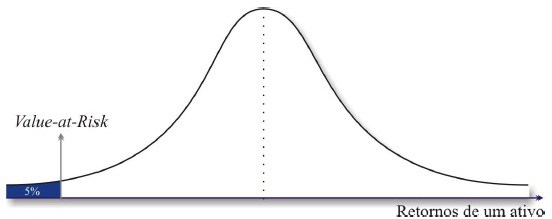
\includegraphics{artigo-var.jpg}
\caption{VaR}
\end{figure}

\end{frame}

\section{Fundamentação Teórica}\label{fundamentacao-teorica}

\begin{frame}{Slide with Bullets}

\begin{itemize}
\tightlist
\item
  Bullet 1
\item
  Bullet 2
\item
  Bullet 3
\end{itemize}

\end{frame}

\section{Modelo}\label{modelo}

\begin{frame}[fragile]{Slide with R Output}

\begin{Shaded}
\begin{Highlighting}[]
\KeywordTok{summary}\NormalTok{(cars)}
\end{Highlighting}
\end{Shaded}

\begin{verbatim}
##      speed           dist       
##  Min.   : 4.0   Min.   :  2.00  
##  1st Qu.:12.0   1st Qu.: 26.00  
##  Median :15.0   Median : 36.00  
##  Mean   :15.4   Mean   : 42.98  
##  3rd Qu.:19.0   3rd Qu.: 56.00  
##  Max.   :25.0   Max.   :120.00
\end{verbatim}

\end{frame}

\begin{frame}{Slide with Plot}

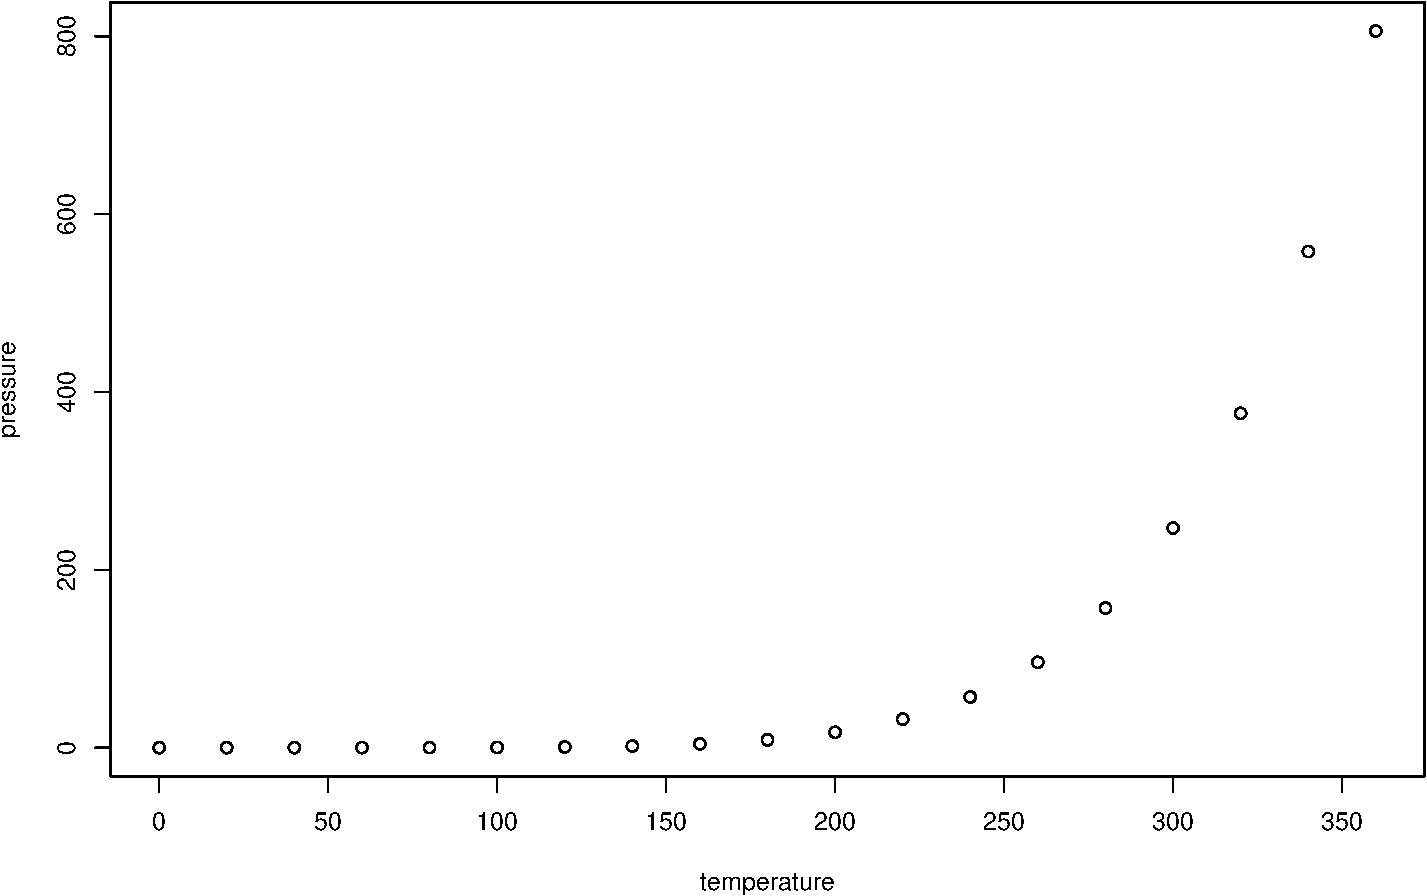
\includegraphics{artigo-apresentacao_files/figure-beamer/pressure-1.pdf}

\end{frame}

\section{Resultados}\label{resultados}

\section{Referências}\label{referencias}

\end{document}
